\chapter{Generators in other platforms}

In this chapter, we will take look at two very different approaches towards supporting generators. First, we will describe the way they are implemented by the C\# compiler Roslyn. The combination of Roslyn and C\# was chosen because, despite the differences between generators in C\# and PHP, it is still very similar to our Peachpie and PHP mix.

Both Roslyn and Peachpie compile their respective languages into the CIL, Peachpie’s compiler is de facto based on Roslyn’s architecture, and generators in PHP are fundamentally a superset of what they are in C\#. 

IronPython and its compiler based on a DLR was also considered, mainly due to Python’s generators being closer to PHP’s. The similarity of compiler platforms and the fact that IronPython offloads a lot of details to the DLR, which is by design generic and therefore needlessly complicated for our use, prevailed, however. 

The second implementation we will talk about in this chapter is Zend Engine’s for generators in PHP. In spite of the fact that we cannot use it as an inspiration, because it relies on a native support provided by the runtime, it is useful to mention it at least briefly. Afterall, it is the implementation we are trying to mimic.

\section{CSharp and Roslyn}\label{sec:3:1}

As said previously, the CIL, into which .NET implementation of C\# gets compiled, does not have a native understanding of generators. There is, for example, no instruction to yield or to automatically construct an iterator type instance with all the appropriate methods. Therefore, the Roslyn compiler has to support generators by lowering them, in essence transforming them into lower level language constructs. 

There are two main components responsible for that. First, there is a rewriter that takes the original generator method and transforms it into a normal method that only uses constructs the CIL supports. We will come back to it later. Then, there is the type implementing the \emph{IEnumerator} interface (\autoref{fig1.1:iterators}), whose instance gets returned from the generator method and which actually represents the generator.


\subsection{Iterator object and generator methods}

There is no single type implementing the \emph{IEnumerator} interface. For each generator method, the Roslyn compiler synthesizes one separate iterator type. While most of their \emph{IEnumerator} methods are simple, and actually the same for all of them, there is one that is always unique - the \emph{next} method. This one actually contains the implementation of the original generator method, only now transformed and turned into a state machine by the rewriter.

The actual original generator method has its body replaced with compiler generated code that instantiates, initiates, and returns the corresponding synthesized type (\autoref{fig4.1:GenMethod}). Therefore, it is a normal CIL method that returns an iterator containing a transformed version of the method’s original body as its \emph{next} method.

\begin{figure}[h]
	\centering	
	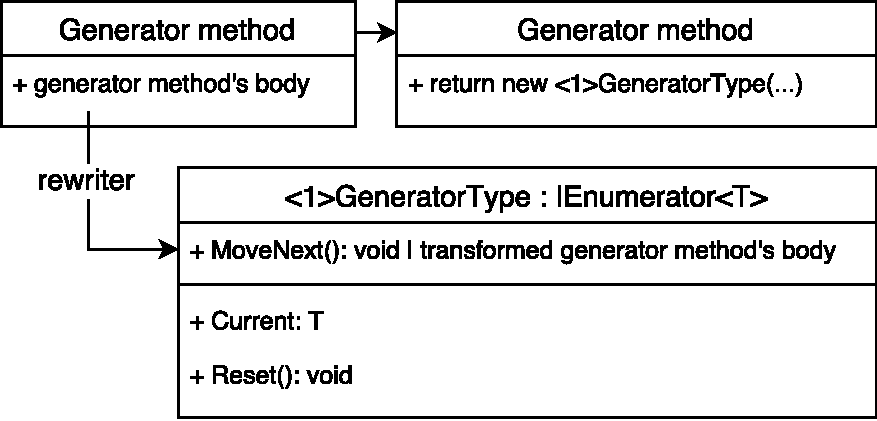
\includegraphics[scale=0.75]{../img/4_1_generatormethods}	
	\caption{Generator method, generator's next method, and the generator type.}
	\label{fig4.1:GenMethod}
\end{figure}

\subsection{Rewriter}

The rewriter has to take care of three things while transforming the original generator method’s body into the iterator’s \emph{next} method. It has fix the references, that expected the method to be where it was instead of on the generated type, and handle both the state saving on yields and the state retrieval in the beginning of the method. 

The only references that care where the method actually is are to \emph{this}. Fortunately, the \emph{this} instance can simply be captured in the original generator method, passed to the generator during its initialization phase, and kept there in a field. All references to the original \emph{this} variable can then be rewritten to references to the generator’s field holding the captured \emph{this} instance.

As for state saving, due to the fact that yield is only a statement in C\# and an invariant in Roslyn, that the evaluation stack is always empty in between separate statements, there are guaranteed to be no temporal values on the stack before any yield gets executed. This means that the only state that needs to be saved are local variables, parameters, and the position, in essence the next statement to be executed.


\subsection{Local variables parameters}

To handle the first two thirds of the state, the rewriter creates a new field on the corresponding iterator type for each local variable and parameter. Then, it replaces all, both read and write, references to these original local variables and parameters with references to the newly created fields (\autoref{fig4.1:LocVars}). The result is that there are no accesses to local variables or parameters in the rewritten method. Also, all values now live on the iterator instance which means they are persistent in between individual calls to the \emph{next} method.

The situation regarding parameters is, in fact, a bit more complicated. As defined by the \emph{IEnumerator} interface, the \emph{next} method cannot have any parameters. Fortunately, there are no references to the parameters inside the \emph{next} method after the rewrite, only to the instance fields they got replaced with. The fields still need to be initialized with their values, however.

That can be done similarly as the this reference was handled in the original generator method. The method has access to both the original parameters and the iterator instance before any code from the \emph{next} method has any chance to access the fields. Hence, after the iterator instance is created, the parameter values get assigned to their corresponding fields as part of an iterator’s initialization phase.

\begin{figure}[h]
	\centering	
	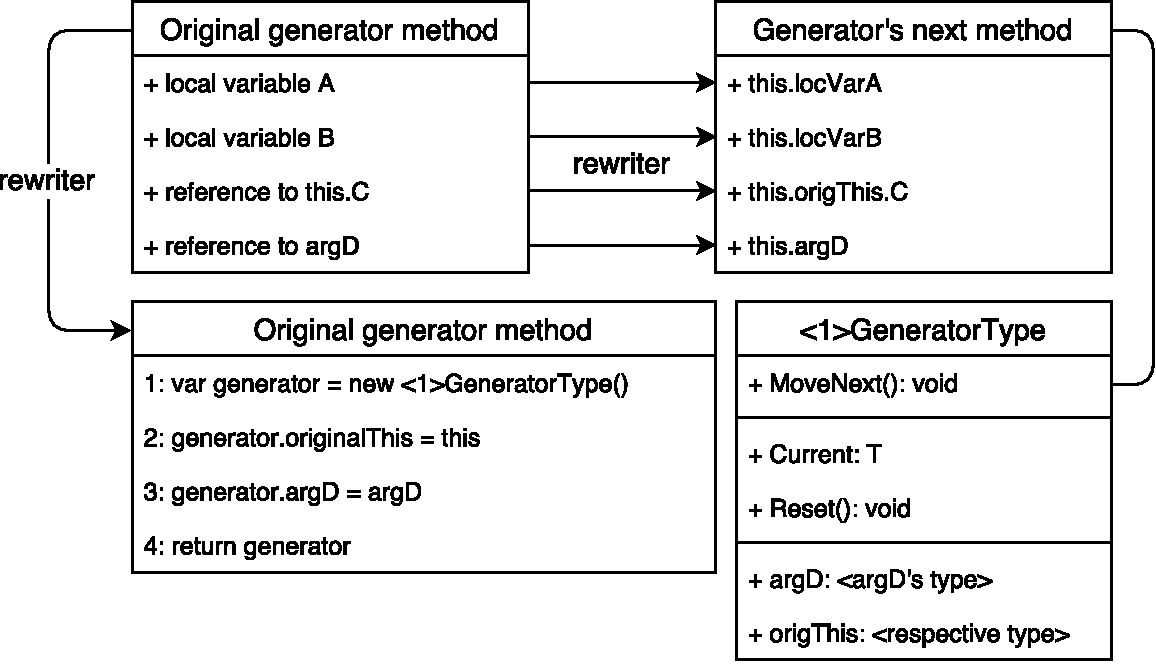
\includegraphics[scale=0.70]{../img/4_1_localVars}	
	\caption{Local variables rewrite for generator methods.}
	\label{fig4.1:LocVars}
\end{figure}

\subsection{Execution position}

The last thing that needs to be taken care of is saving the point where the last yield happened, effectively the place a subsequent call of the \emph{next} method should continue from. To handle that, the rewriter does two main things. It replaces each \emph{yield} with a number of statements and creates a jump table in the beginning of the \emph{next} method (\autoref{fig4.1:Position}). A new field called state, representing which yield the generator exited with last time, is also created on the iterator instance.

Each \emph{yield} gets lowered into four separate statements. First, an assignment of the yielded value to a current field on the iterator instance. This field is used by the \emph{IEnumerator}'s \emph{current} method as its backing field. Second, an assignment of the current \emph{yield}’s index to a state field on the iterator instance. The order of these indexes can be arbitrary, only a uniqueness among other \emph{yield}s' indexes within the same method is required. Third, a normal \emph{return} from the \emph{next} method. And finally, a \emph{yield}’s label based on its index that can be used as a target for jumps.

The jump table in the beginning of the \emph{next} method is fundamentally a switch statement that, based on the current value of the iterator’s state field, jumps to a corresponding \emph{yield}'s label. Within the four statements created by rewriting one yield, the state field assignment and the label are connected. The assignment sets a state value whose corresponding case in the switch table contains a jump to the label. And since the indexes and therefore states are unique, it is guaranteed that this always holds true.

\begin{figure}[h]
	\centering	
	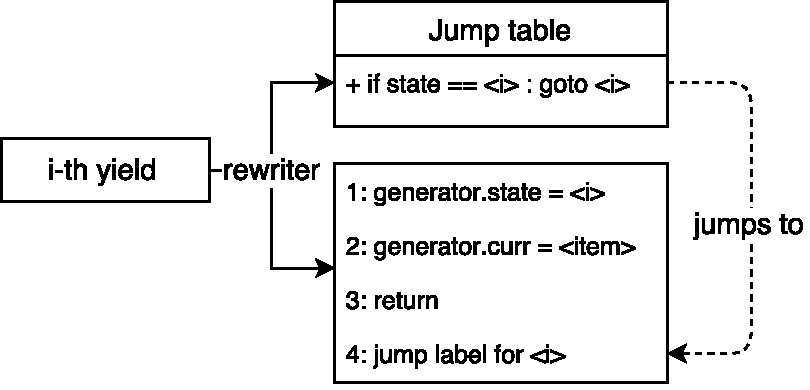
\includegraphics[scale=0.75]{../img/4_1_position}	
	\caption{Local variables rewrite for generator methods.}
	\label{fig4.1:Position}
\end{figure}

That way when the \emph{next} method is called repeatedly, it always resumes with the statement that is directly after the \emph{return} the method exited with before. This happens simply due to the fact that whenever you hit a \emph{yield}, and therefore a \emph{return}, two things are true. 

First, just before returning from the \emph{next} method, an index of the hit \emph{yield} gets assigned to the state field. Second, the state field does not change unless the \emph{next} method is called again. And when that happens, the switch table in the beginning of the \emph{next} method jumps to the label that was created by rewriting the same \emph{yield} as the last evaluated state assignment. Which is, as we have already proven, the label directly after the \emph{return} the method exited with previously.

\begin{listing}[H]
\caption{Original and rewritten generator method's body.}
\label{list4.1:generatorRewrite}
\begin{minted}{csharp}
// Original method's body
Yield 5;
Yield 10;

// New method's body
switch(this.state){
  case 1:
    goto: Label_1;
    break;
  case 2:
    goto: Label_2;
    break;
}

this.current = 5;
this.state = 1;
return;
Label_1;

this.current = 10;
this.state = 2;
return;
Label_2;
\end{minted}
\end{listing}

Naturally, this is not all the Roslyn compiler does to support generators in C\#. It is, however, more than enough for us to design our own implementation in the Peachpie compiler. 


\section{PHP and Zend Engine}

Unlike CIL and CLR respectively, the reference PHP runtime Zend Engine understands generators natively \citep{ZendGen}. As such, it is able to execute yields without having to lower them into simpler PHP constructs.

Not going into details and slightly simplifying, the execution state of the Zend engine is represented by a virtual machine stack. This stack contains individual stack frames, each corresponding to a method’s execution. When a method is called, a new stack frame gets created, initiated, and pushed on top of the stack. When the method returns, its stack frame gets popped.

Each frame contains the complete information about a method’s execution state, all of its local and temporal variables, arguments, the returned value, and an index of the last executed statement, to name a few. Therefore, if one needed to save the execution state of a method, storing its frame stack would be enough.

And that is exactly what the Zend engine does when it encounters a yield expression. It creates a new generator object, copies the current stack frame into it, performs a number of other tasks, such as setting its current key and value, and finally returns the iterator. In this context, the current stack frame is the one representing the execution state of the method with yields and therefore, in essence, the generator method.

Later, when the \emph{next} method is called on the returned generator instance, it restores the stack frame previously saved on the generator object to the top of the virtual machine stack and resumes the execution. This effectively causes the generator method’s execution to continue from the very point where the last yield was encountered and thus where it stopped. On subsequent yields, the runtime sets the generator’s fields such as key and current, updates its saved stack frame representing the generator method's current state, and returns.

The description above is a simplification of the actual process that happens in the Zend engine, with details regarding yields in exception blocks and inside function calls completely omitted. However, it still provides a good high level overview of how generators are implemented in PHP’s reference runtime and how it is different to Roslyn’s approach.  
